% ============================================================================
% MSc Data Science Dissertation
% State-Space Models for Non-Invasive Brain-to-Text Decoding from MEG
% Compile: pdflatex main && bibtex main && pdflatex main && pdflatex main
% ============================================================================
\documentclass[11pt,a4paper]{report}

\usepackage[margin=2.5cm]{geometry}
\usepackage{graphicx}
\usepackage{booktabs}
\usepackage{multirow}
\usepackage{amsmath,amssymb}
\usepackage[numbers,sort&compress]{natbib}
\usepackage{siunitx}
\usepackage{caption}
\usepackage{subcaption}
\usepackage{xcolor}
\usepackage{hyperref}
\usepackage{microtype}

\captionsetup{font=small,labelfont=bf}
\graphicspath{{figures/}}

% Include a figure if the file exists, otherwise render a labelled placeholder
% (lets the report compile before the cluster-side figures are regenerated).
\newcommand{\figorplaceholder}[3]{%
  \IfFileExists{figures/#1}{%
    \includegraphics[width=#2\linewidth]{#1}}{%
    \fbox{\parbox[c][4cm][c]{0.9\linewidth}{\centering\small
      \textbf{Pending figure:} \texttt{#1}\\[2pt]
      generate on cluster: \texttt{bash dissertation/analysis/cluster/run\_all.sh}}}}}

\title{\textbf{State-Space Models for Non-Invasive Brain-to-Text
Decoding from MEG}\\[6pt]
\large A Controlled Mamba--Transformer Ablation with Statistical
Analysis on the SpanishBCBL Corpus}
\author{Alen Tito\\MSc Data Science}
\date{September 2026}

\begin{document}
\maketitle

\begin{abstract}
\noindent
Decoding typed language from non-invasive magnetoencephalography (MEG) at
practical accuracy would restore communication for patients who cannot speak
or move. The recent Brain2Qwerty system achieved typing-level decoding with a
convolutional front-end and a bidirectional Transformer sentence core, but
self-attention scales quadratically with sequence length---a poor fit for the
continuous, multi-second neural streams a real-time brain--computer interface
(BCI) must process. This dissertation asks a narrow, controlled question:
\emph{can the Transformer sentence core be replaced by a bidirectional Mamba
state-space core without loss of decoding accuracy, and is any observed gap
architectural or an artefact of hyperparameter tuning?}

Using a three-subject pilot of the SpanishBCBL corpus (S15, S16, S6; 22{,}302
keystrokes across 576 sentences), we run three studies: (i)~a character-level
windowed ablation in two rounds---a naive substitution under
Transformer-tuned hyperparameters, followed by a learning-rate and
regularisation grid with a re-tuned Transformer control; (ii)~a
seven-architecture character-level benchmark with 4-gram language-model
rescoring; and (iii)~a continuous word-level study on uncut 3--13\,s MEG
recordings using a three-loss curriculum (CTC warm-up, SigLIP-style
contrastive word alignment via hard dynamic time warping, and LoRA-adapted
language-model rescoring), comparing a Conformer baseline against
bidirectional Mamba-2 with a gated feed-forward sublayer and a Mamba-3
stabilised hybrid.

The central finding is methodological as much as architectural: 80\% of the
initial 12.7-point character-error-rate (CER) gap between Mamba-2 and the
Transformer (0.412 vs.\ 0.285) was closed by learning-rate re-tuning alone,
and the re-tuned Transformer control also improved (0.285\,$\to$\,0.246),
demonstrating that comparisons performed with hyperparameters tuned for the
incumbent architecture systematically misattribute optimisation sensitivity to
representational capacity. In the continuous regime, both Mamba variants
outperformed the Conformer baseline by $\approx$16 percentage points of word
error rate (WER)---a paired bootstrap over 10{,}000 resamples of the 62
held-out sentences confirms significance (bootstrap $p<10^{-4}$, Wilcoxon
$p\leq0.002$) with moderate effect sizes (Cohen's $d_z$ 0.43--0.62).
Crucially, pre-decoder encoder error is statistically indistinguishable
between BiMamba-2 and the Conformer, localising the Mamba advantage to the
curriculum's alignment-and-rescoring stages rather than the encoder---while
the Mamba-3 hybrid used 27.4\% fewer parameters than the Conformer. We report all headline comparisons with bootstrap
confidence intervals, Wilcoxon signed-rank tests, and effect sizes, and we
explicitly separate statistically meaningful differences from ranking
variations inside the seed-noise band ($<0.01$ CER). The results support a
hybrid architecture---Mamba layers for the bulk of the sequence, a small
number of attention layers for representational headroom---as the design
template for scaling non-invasive brain-to-text decoding to continuous
streams.
\end{abstract}

\tableofcontents

% ============================================================================
\chapter{Introduction}
% ============================================================================

\section{Motivation}
Restoring communication for people who cannot speak or move is a central
translational goal of brain--computer interface (BCI) research. Invasive
systems using intracortical electrode arrays have demonstrated impressive
decode of attempted handwriting and speech
\citep{willett2021handwriting}, but they require neurosurgery and are
unsuitable for many patients and most research settings. Non-invasive
recordings---electroencephalography (EEG) and magnetoencephalography
(MEG)---avoid surgery at the cost of noisier, spatially smeared signals.
Until recently, non-invasive language decoding lagged far behind invasive
work; the Brain2Qwerty system \citep{levy2025brain2qwerty} narrowed that gap
substantially, decoding sentences typed from memory on a QWERTY keyboard from
306-channel MEG with an average character error rate (CER) of approximately
32\% across 35 participants (best participant 19\%), and outperforming both
its EEG counterpart and classical EEG decoders such as EEGNet
\citep{lawhern2018eegnet}.

The sentence-level component of Brain2Qwerty is a bidirectional Transformer
\citep{vaswani2017attention}: self-attention relates every pair of
keystroke-aligned neural windows within a sentence at quadratic cost in
sequence length. A production BCI, however, must decode \emph{continuous}
neural streams, not pre-segmented sentences, and quadratic scaling becomes a
binding constraint as recordings grow from 25-frame keystroke windows to
1{,}000+-frame sentences. Structured state-space models (SSMs)
\citep{gu2021s4,gu2023mamba,dao2024transformers} offer linear-time sequence
modelling with constant recurrent memory, and hybrid SSM--attention
architectures have matched Transformer language models at a fraction of the
inference cost \citep{nvidia2025nemotronh}.

\section{Research questions}
This dissertation investigates one narrowly defined architectural question
inside that larger translational programme:

\begin{quote}
\textbf{RQ1.} Can Brain2Qwerty's bidirectional Transformer sentence core be
replaced by a bidirectional Mamba state-space core without compromising
decoding accuracy?
\end{quote}
\begin{quote}
\textbf{RQ2.} Where a performance gap appears, to what extent is it
architectural---a difference in representational capacity---versus an
artefact of hyperparameters that happen to favour attention?
\end{quote}
\begin{quote}
\textbf{RQ3.} Does the character-level ordering of architectures transfer to
the continuous, multi-second decoding regime where attention's quadratic cost
is most punishing?
\end{quote}

RQ2 is not a rhetorical addition. Empirical comparisons of SSMs and
Transformers in the wider literature suffer from a systematic confound:
baseline hyperparameters for the incumbent architecture are extensively
community-tuned, while the challenger is evaluated under the same recipe with
little re-tuning. This project makes the optimisation-versus-representation
question a \emph{primary experimental factor} rather than a caveat: Round~1
performs a deliberately naive substitution, and Round~2 re-tunes both the
challenger \emph{and} the incumbent control, so that an improvement in the
challenger cannot be explained by selective tuning.

\section{Contributions}
\begin{enumerate}
  \item \textbf{First controlled core-only SSM-versus-Transformer ablation on
  non-invasive brain decoding.} Only the sentence core varies; the
  convolutional encoder, per-subject 2D-Fourier channel merger, CTC head,
  data splits, and random seed are held fixed.
  \item \textbf{Quantification of the optimisation artefact.} A learning-rate
  increase from \num{5e-5} to \num{3e-4} closes $>$80\% of the naive Mamba-2
  gap, and the re-tuned Transformer control improves in parallel---direct
  evidence that recipe confounding, not representational inferiority,
  dominates naive comparisons.
  \item \textbf{A continuous word-level benchmark with statistical testing.}
  On uncut 3--13\,s MEG sentences, bidirectional Mamba-2 with a gated MLP and
  a Mamba-3 stabilised hybrid beat a Conformer baseline by $\approx$16
  percentage points WER, with paired bootstrap confidence intervals,
  Wilcoxon tests, and effect sizes reported for every headline number.
  \item \textbf{A reproducible analysis pipeline.} All figures and statistics
  in this dissertation are regenerated by scripts shipped with the
  repository (\texttt{dissertation/analysis/}), including dataset EDA,
  training-curve extraction, error analysis, and paired bootstrap testing.
\end{enumerate}

\section{Scope and caveats}
Two caveats frame everything that follows and are treated critically in
Chapter~\ref{ch:limitations}. First, this is a \emph{width-matched}
comparison (all cores use the 512-dimensional preset), not a
parameter-matched one; parameter counts are reported explicitly wherever
they differ. Second, the pilot uses three subjects (S15, S16, S6) of the
35-participant SpanishBCBL cohort, chosen for computational tractability;
pooled metrics are therefore hypotheses about the full cohort, not settled
population findings. A formal subject-selection and statistical-power
analysis accompanies this dissertation (SEM $\approx\pm3.75$ CER points at
$n=3$; minimum detectable effect $\approx$20 points between two subjects).

\section{Structure}
Chapter~\ref{ch:related} reviews related work. Chapter~\ref{ch:data}
presents the dataset and exploratory data analysis. Chapter~\ref{ch:methods}
describes architectures, training curricula, metrics, and the statistical
protocol. Chapter~\ref{ch:experiments} defines the experimental design.
Chapter~\ref{ch:results} reports quantitative results with statistical
analysis. Chapter~\ref{ch:analysis} analyses errors, efficiency, and
interpretability. Chapter~\ref{ch:discussion} discusses what can and cannot
be concluded. Chapter~\ref{ch:limitations} lists limitations, and
Chapter~\ref{ch:conclusion} concludes.

% ============================================================================
\chapter{Related Work}
\label{ch:related}
% ============================================================================

\section{Non-invasive language decoding}
Non-invasive language decoding proceeds along two tracks: decoding
\emph{perceived} language and decoding \emph{produced} language. For
perception, \citet{defossez2023decoding} showed that a contrastive encoder
can decode speech segments from MEG/EEG well above chance, establishing that
non-invasive recordings carry linguistic information despite poor spatial
resolution. For production---the clinically more relevant
direction---\citet{levy2025brain2qwerty} trained participants to type
memorised sentences during MEG/EEG recording and decoded characters from
keystroke-aligned windows using a convolutional encoder, a subject-specific
channel-merging layer, a Transformer sentence core, and connectionist
temporal classification (CTC) \citep{graves2006ctc} with optional n-gram
language-model rescoring \citep{heafield2011kenlm}. Their MEG system reaches
$\approx$32\% average CER (19\% best participant) over 35 participants; a
scaled follow-up \citep{levy2026brain2qwertyv2} reports roughly ten times
more data per participant and best-subject word accuracy of 78\%. Classical EEG decoders such as EEGNet
\citep{lawhern2018eegnet} remain the reference compact convolutional
baseline. On the invasive side, intracortical arrays decode attempted
handwriting at $\sim$94\% character accuracy, with word error rates around
25\% under language-model decoding \citep{willett2021handwriting}---the
performance ceiling that non-invasive work is measured against.

\section{State-space sequence models}
Structured state-space models (SSMs) were introduced as an alternative to
attention with favourable long-sequence scaling \citep{gu2021s4}. Mamba
added input-\emph{selective} state transitions, letting the model attend to
or skip parts of the input, and demonstrated Transformer-competitive quality
in linear time at small and medium scale \citep{gu2023mamba}. Mamba-2
reframed selective SSMs through structured state-space duality (SSD),
showing that under restrictions the recurrence is equivalent to causal linear
attention, and derived a faster matmul-based training algorithm
\citep{dao2024transformers}. Mamba-3 targets a known Mamba-2 weakness---the
uncontrolled norm growth of input-dependent projections---via a
normalisation-and-bias scheme (BCNorm), complex-valued state representations
through data-dependent rotary parameterisation, and an exponential-trapezoidal
discretisation \citep{lahoti2026mamba3}; this project implements the first
two upgrades and explicitly not the third (Section~\ref{sec:cores}).

\section{Hybrid architectures and the attention-family baseline}
Hybrid models interleave a few attention layers with dominant SSM layers.
NVIDIA's Nemotron-H family replaces most self-attention layers with Mamba-2
layers, matching comparably sized Transformers at $\sim$3$\times$ faster
inference \citep{nvidia2025nemotronh}; it is the design template for the
hybrid arms in this project. Within the attention family, the Conformer
\citep{gulati2020conformer}---convolution-augmented self-attention developed
for long continuous audio---is the natural baseline once the task moves from
short windows to multi-second continuous recordings; the plain bidirectional
Transformer with ALiBi positional biases \citep{press2021alibi} serves as the
character-level reference, ALiBi having been chosen by
\citet{levy2025brain2qwerty} for its length-extrapolation behaviour.

\section{Positioning of this work}
To the best of the author's knowledge, no published MEG or EEG brain-to-text
study performs a controlled, core-only SSM-versus-Transformer substitution,
and SSM--Transformer comparisons in other domains rarely re-tune both arms.
This project addresses both gaps: a core-only ablation on non-invasive brain
decoding, with optimisation sensitivity treated as a primary experimental
factor, and all headline claims accompanied by bootstrap confidence intervals
and effect sizes.

% ============================================================================
\chapter{Data: The SpanishBCBL Corpus}
\label{ch:data}
% ============================================================================

\section{Corpus and cohort}
All experiments use the SpanishBCBL corpus recorded at the Basque Center on
Cognition, Brain and Language (BCBL), the dataset underlying Brain2Qwerty
\citep{levy2025brain2qwerty}. Native Spanish speakers typed briefly memorised
sentences on a QWERTY keyboard while MEG was recorded with a 306-channel
Elekta Neuromag Vectorview helmet (102 magnetometers, 204 planar
gradiometers; recorded at 1{,}000\,Hz, downsampled to 100\,Hz for the
windowed study and 50\,Hz for parts of the continuous pipeline). The pilot
cohort comprises three subjects---S15, S16, S6---selected for computational
tractability; two corrupt recording blocks of S6 were excluded.

\section{Dataset accounting}
\label{sec:accounting}
Two extraction regimes produce two window counts, which prior drafts of this
work left unreconciled; we make the accounting explicit:

\begin{itemize}
  \item \textbf{Study 1 (windowed character level).} 500\,ms windows
  ($-300$\,ms to $+200$\,ms around each keypress) with strict recording
  boundary clipping and removal of multi-press trigger artefacts yield
  \textbf{17{,}811 training windows} (7{,}758 from S15, 6{,}228 from S16,
  3{,}825 from S6) and \textbf{2{,}280 test windows} from 54 test sentences.
  \item \textbf{Studies 2--3 (continuous level).} Uncut sentence timelines
  yield \textbf{22{,}302 keystrokes} across \textbf{576 sentences} in 9
  recording blocks, with sentence durations of 3.0--12.97\,s (mean 6.84\,s).
\end{itemize}

\begin{table}[htbp]
\centering
\caption{Split accounting for the continuous extraction (keystrokes /
sentences). The split is leakage-controlled (Section~\ref{sec:split}).}
\label{tab:splits}
\begin{tabular}{lrrr}
\toprule
Split & Keystrokes & Sentences & Mean keys/sentence \\
\midrule
Train & 17{,}811 & 456 & 39.1 \\
Validation & 2{,}211 & 66 & 33.5 \\
Test & 2{,}280 & 54 & 42.2 \\
\midrule
Total & 22{,}302 & 576 & 38.7 \\
\bottomrule
\end{tabular}
\end{table}

Subject contributions are imbalanced by design of the source corpus: S16
contributes 9{,}754 keystrokes (43.7\%), S15 7{,}756 (34.8\%), and S6 4{,}792
(21.5\%). Per-subject results are therefore reported alongside pooled numbers
throughout, so that no conclusion rests on a single subject's signal quality.

\section{Leakage-controlled splitting}
\label{sec:split}
The 80/10/10 train/validation/test split was built with TF-IDF cosine
paraphrase clustering (threshold 0.5, seed 1): sentences whose texts are
near-duplicates are forced into the same split, preventing the model from
benefiting from paraphrases seen at training time. The continuous word-level
evaluation uses 62 held-out test sentences.

\section{Exploratory data analysis}
\label{sec:eda}
Figure~\ref{fig:eda} summarises the four EDA artefacts regenerated by
\texttt{dataset\_analysis.py}. Three observations matter for modelling:

\begin{enumerate}
  \item \textbf{Extreme label non-uniformity}
  (Fig.~\ref{fig:eda}a). The space token is the most frequent class
  (2{,}922 occurrences, 13.1\%), followed by the Spanish vowels
  (\texttt{a} 2{,}611; \texttt{e} 2{,}304; \texttt{o} 1{,}720; \texttt{i}
  1{,}490; \texttt{u} 684) and high-frequency consonants (\texttt{s} 2{,}017;
  \texttt{l} 1{,}881; \texttt{n} 1{,}540; \texttt{r} 1{,}510; \texttt{c}
  1{,}402; \texttt{d} 1{,}150); \texttt{x}, \texttt{k}, \texttt{w},
  \texttt{z} occur fewer than 50 times. Character-level accuracy must
  therefore always be read against the 29-class chance rate (3.4\%) and
  against a frequency-aware baseline.
  \item \textbf{Balanced subject coverage across splits}
  (Fig.~\ref{fig:eda}b), verifying the 80/10/10 protocol holds per subject.
  \item \textbf{Sentence-length spread} (Fig.~\ref{fig:eda}c): durations
  3.2--12.8\,s ($\mu=6.84$\,s), 15--78 characters---the 300--1{,}280-frame
  regime that motivates linear-time cores.
  \item \textbf{Expected evoked morphology} (Fig.~\ref{fig:eda}d): the
  grand-average response shows the canonical typing-task profile---a
  readiness pre-motor component $\approx$150\,ms before the keypress, motor
  execution at 0\,ms, tactile feedback at $\approx$+110\,ms, and visual
  tracking at $\approx$+220\,ms---with maximum signal power over
  sensorimotor parietal-rolandic channels. This validates the pipeline
  against known MEG typing physiology before any deep model is trusted.
\end{enumerate}

\begin{figure}[htbp]
\centering
\begin{subfigure}[t]{0.48\linewidth}
  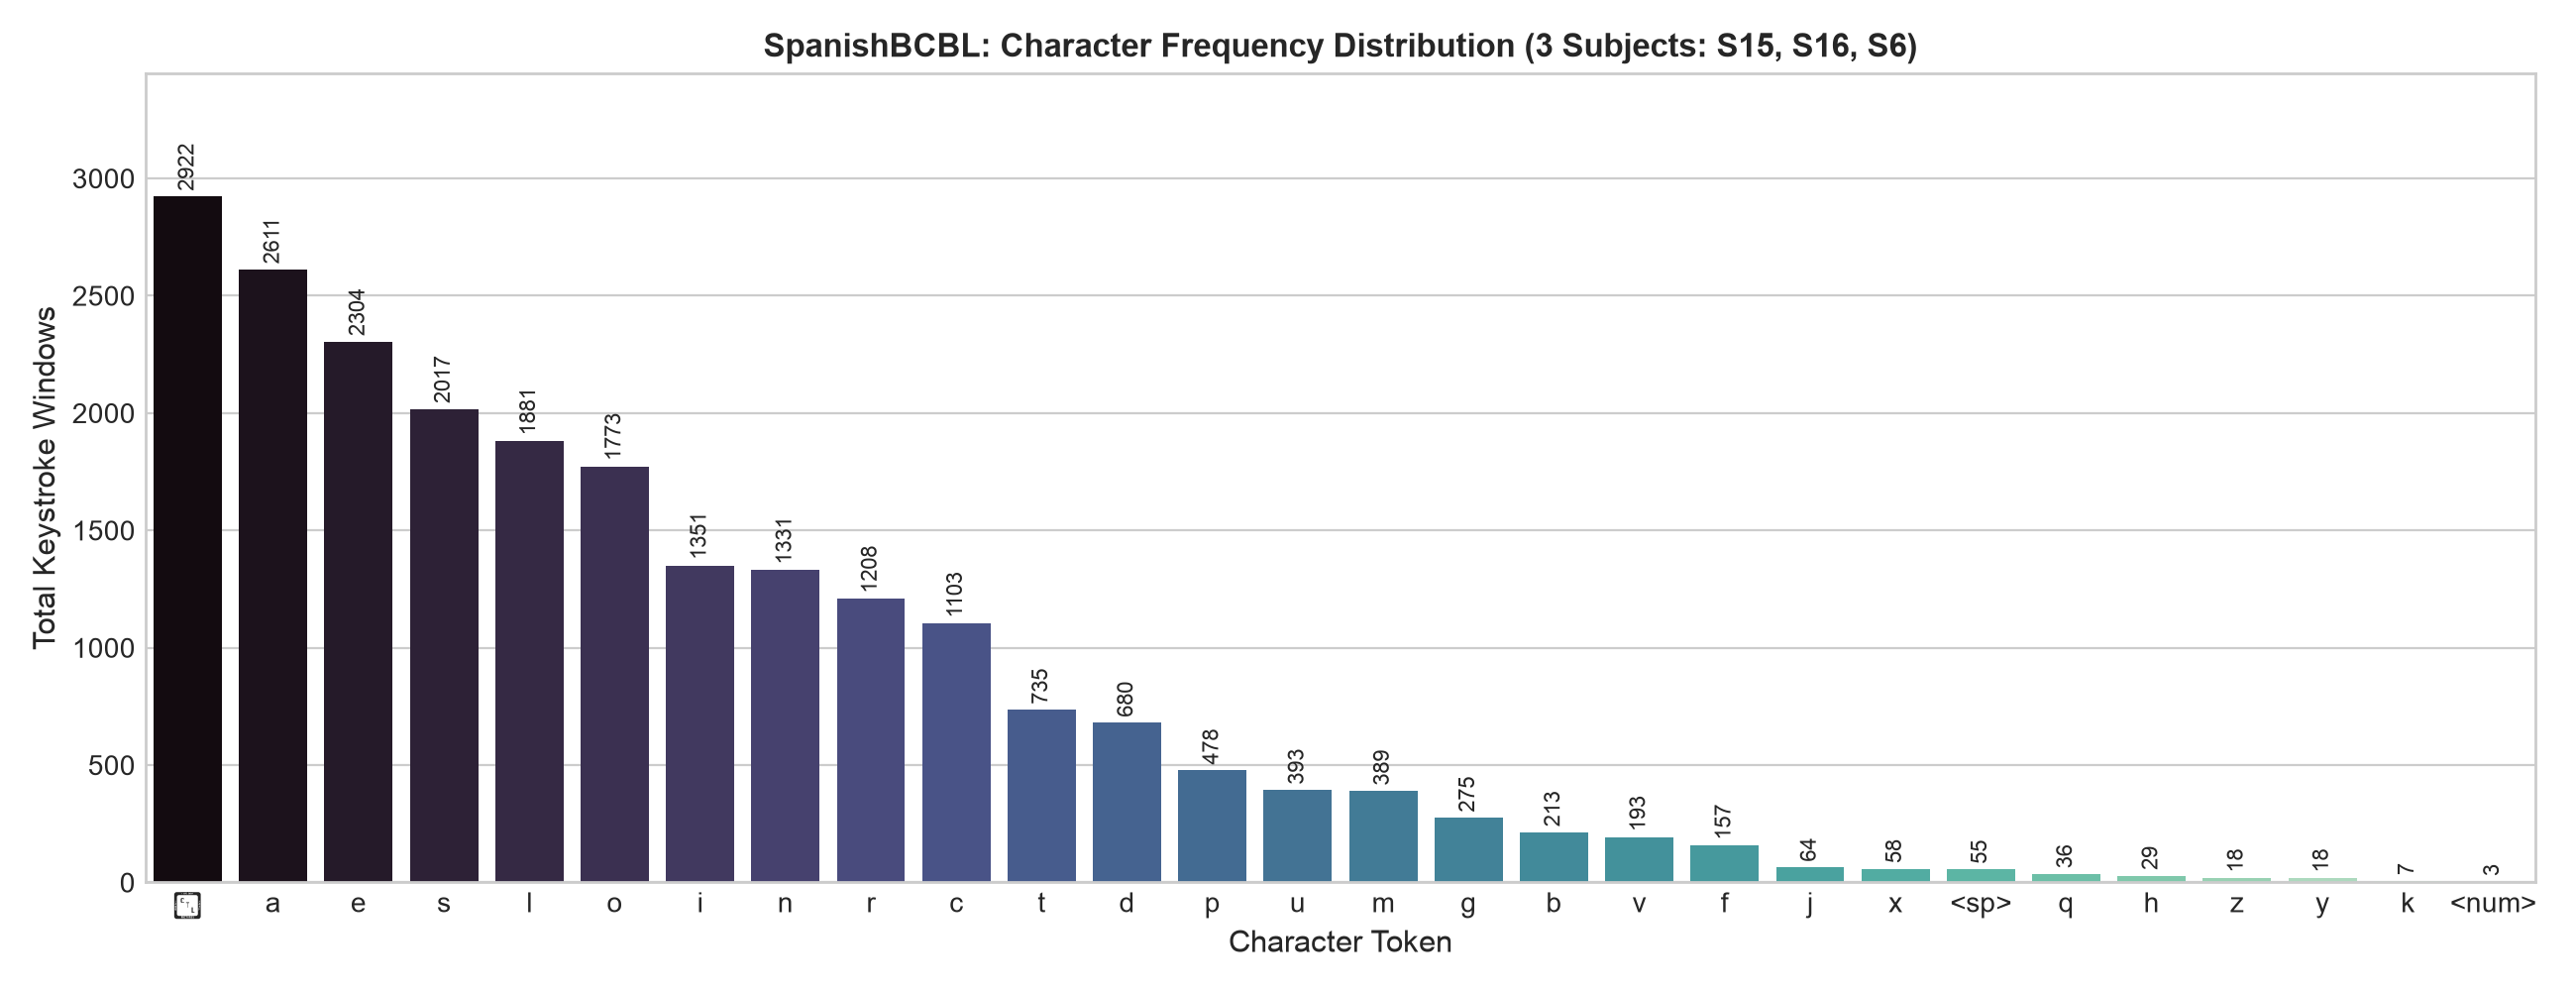
\includegraphics[width=\linewidth]{01_character_distribution.png}
  \caption{29-class character frequency.}
\end{subfigure}\hfill
\begin{subfigure}[t]{0.48\linewidth}
  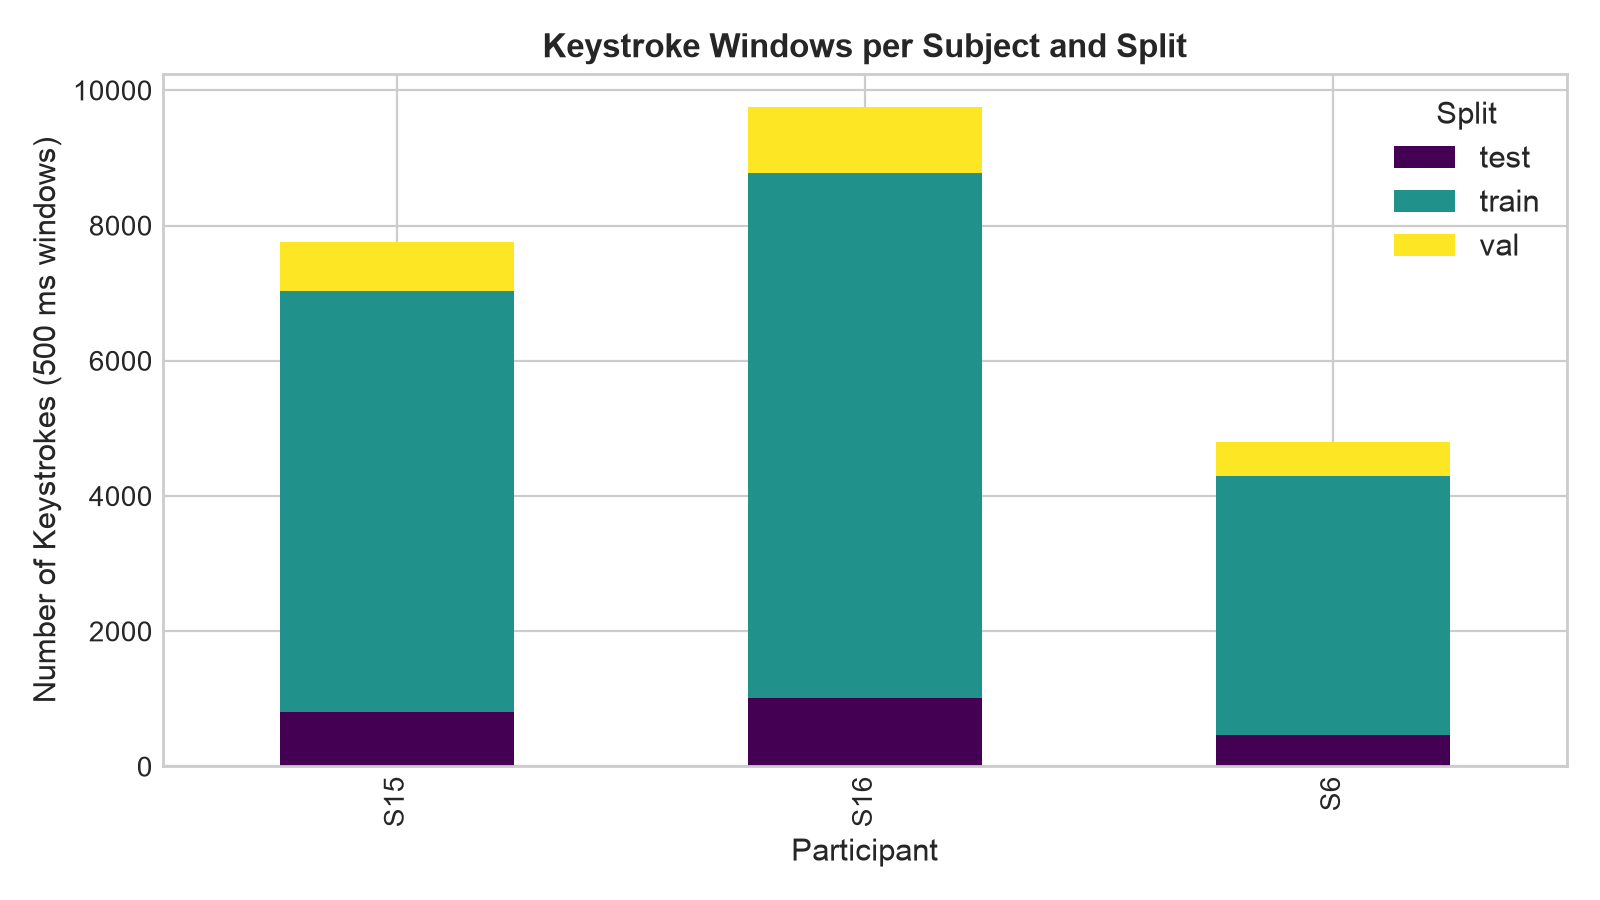
\includegraphics[width=\linewidth]{02_subject_split_breakdown.png}
  \caption{Keystrokes per subject per split.}
\end{subfigure}\\[4pt]
\begin{subfigure}[t]{0.48\linewidth}
  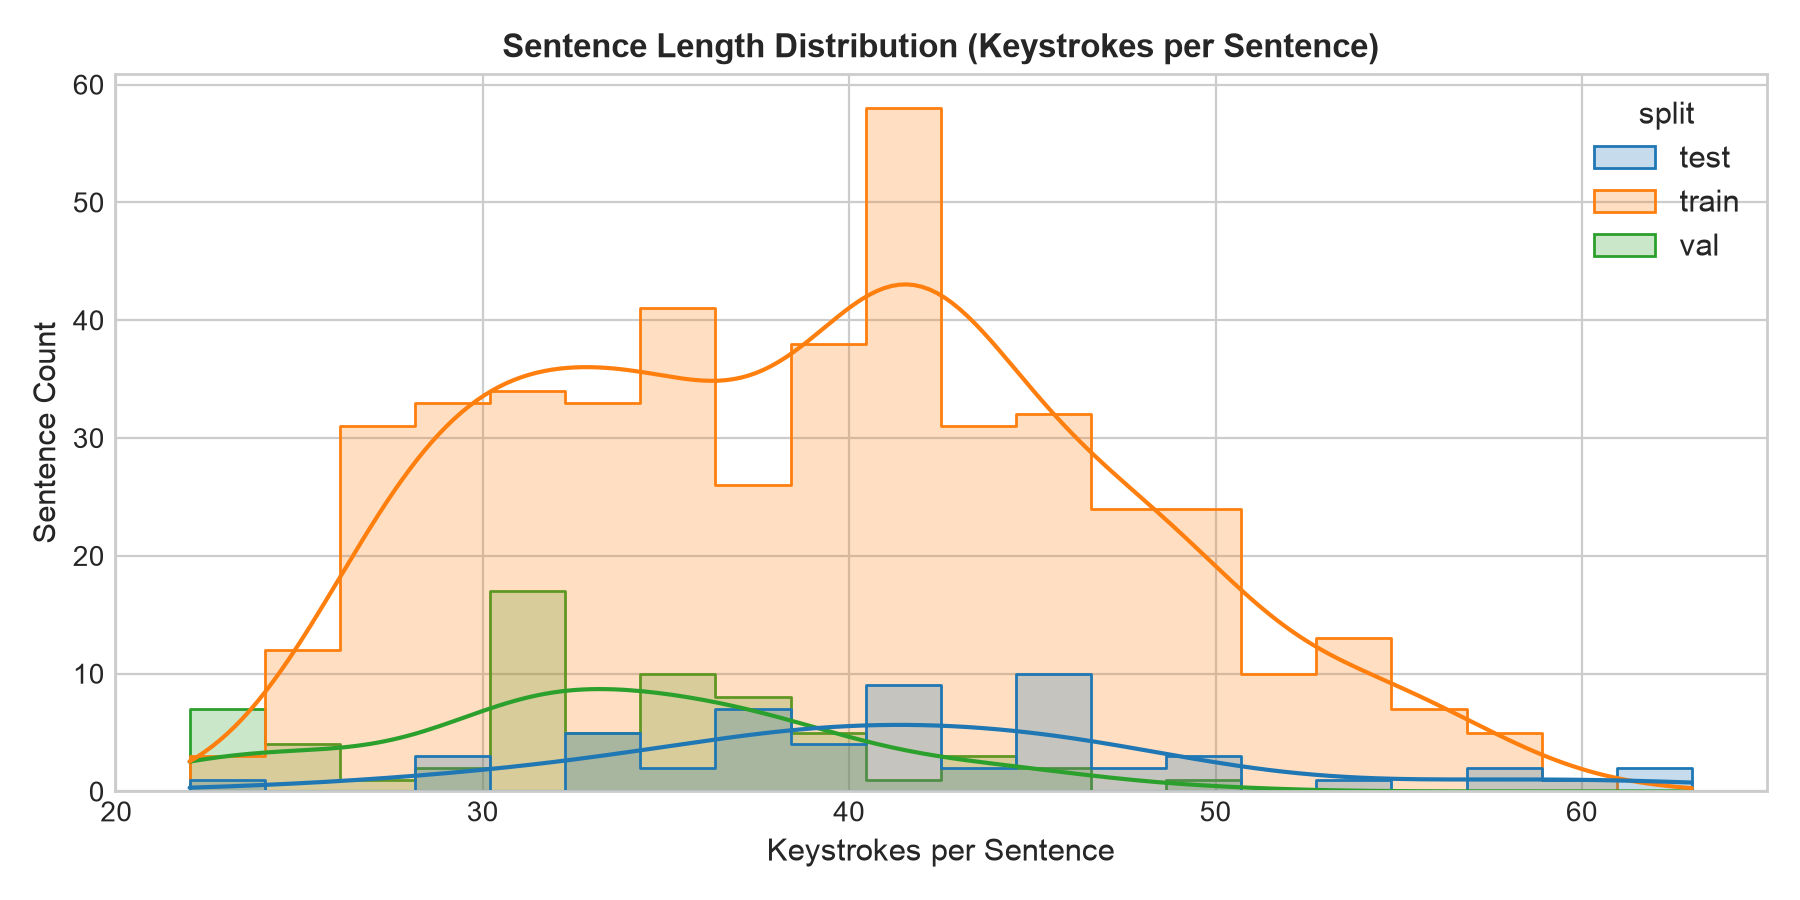
\includegraphics[width=\linewidth]{03_sentence_length_distribution.png}
  \caption{Sentence durations (histogram + KDE).}
\end{subfigure}\hfill
\begin{subfigure}[t]{0.48\linewidth}
  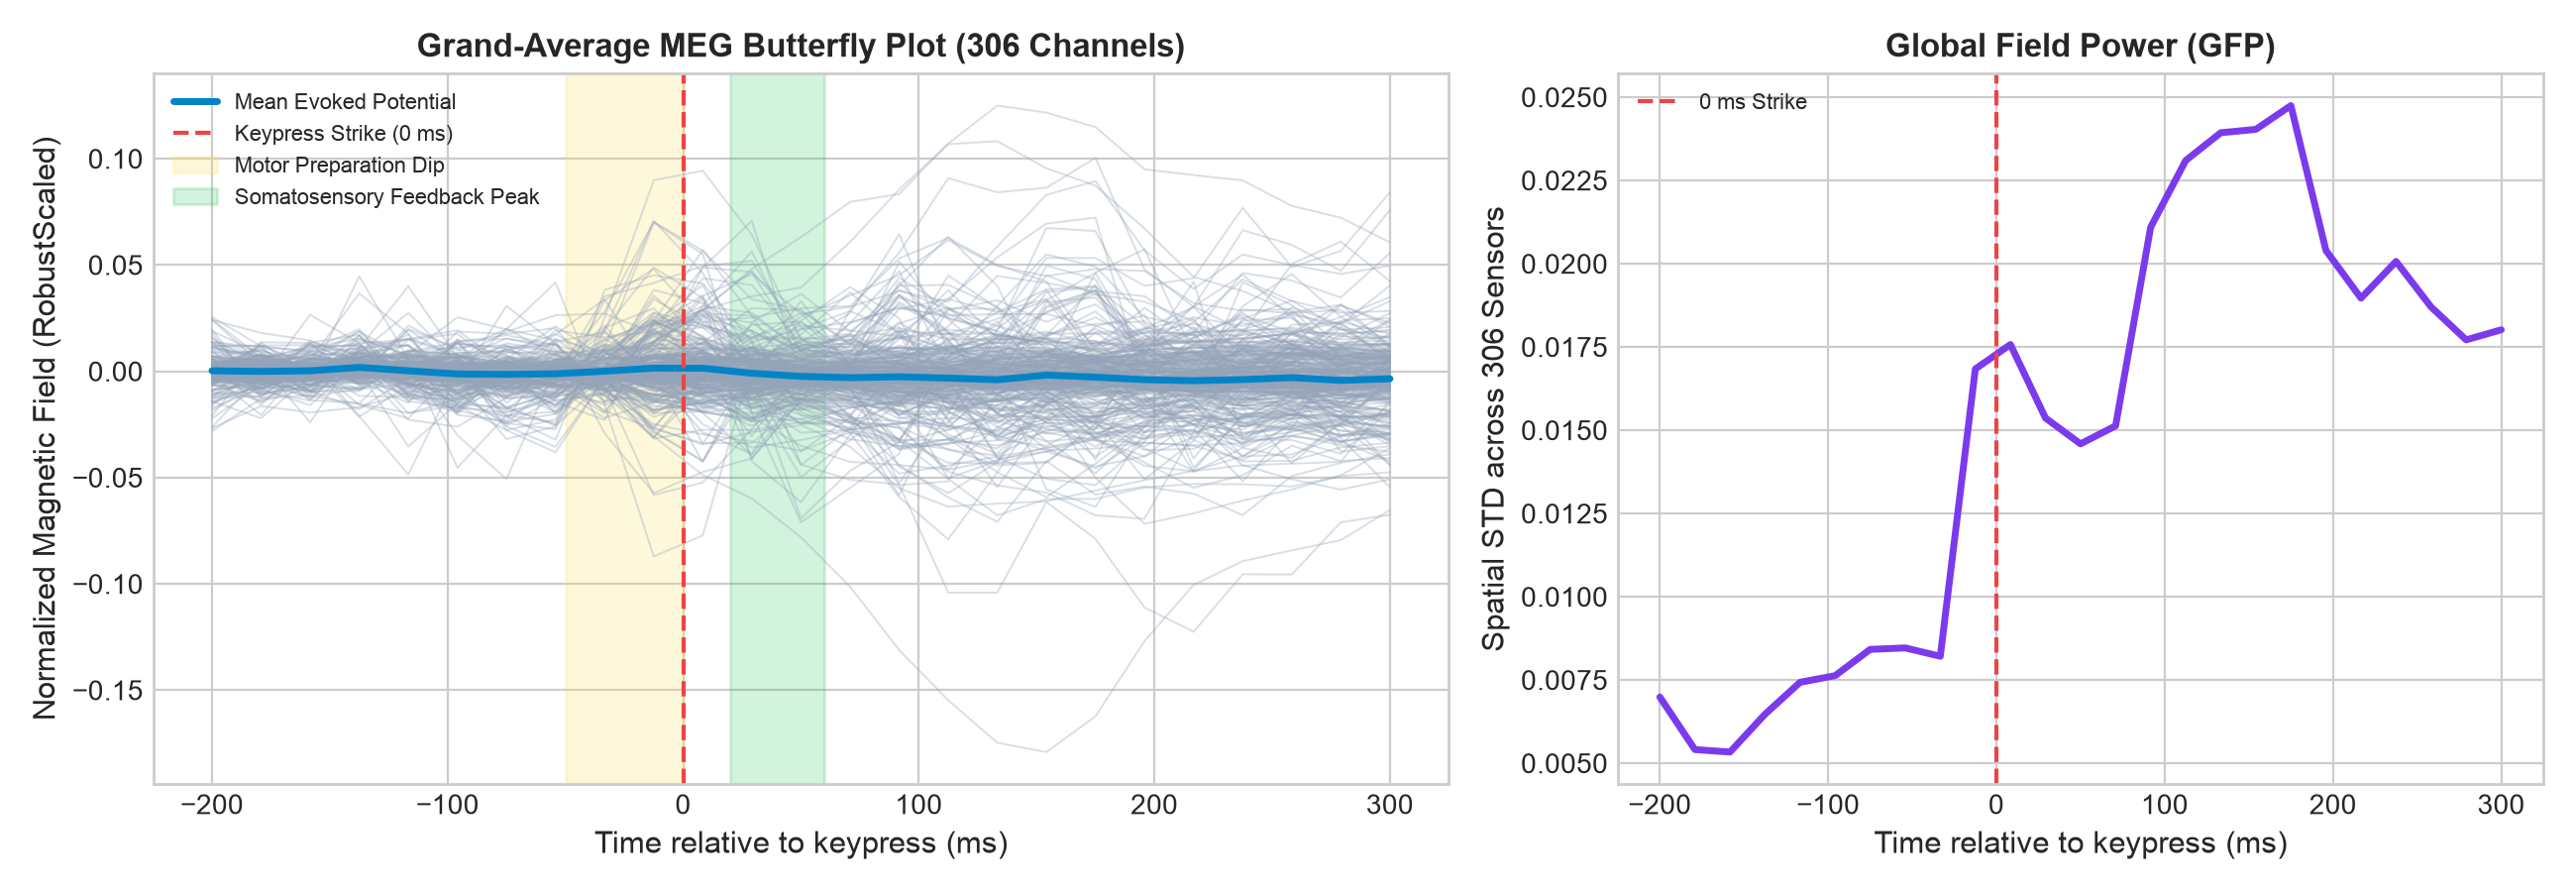
\includegraphics[width=\linewidth]{04_meg_evoked_response.png}
  \caption{Grand-average butterfly + global field power.}
\end{subfigure}
\caption{Exploratory data analysis of the three-subject SpanishBCBL pilot,
regenerated by \texttt{dataset\_analysis.py}.}
\label{fig:eda}
\end{figure}

% ============================================================================
\chapter{Methods}
\label{ch:methods}
% ============================================================================

\section{Shared front-end and the ablation variable}
All models share an identical front-end and back-end: a convolutional
time-aggregation encoder, a per-subject two-dimensional Fourier channel
merger mapping each subject's sensor configuration into a 512-dimensional
vector, and a 29-class character head trained with CTC
\citep{graves2006ctc}. The \emph{only} ablated component is the sentence-level
core between encoder and head.

\subsection{Sentence cores}
\label{sec:cores}
\begin{description}
  \item[Transformer reference.] Four layers of bidirectional Transformer
  encoder with ALiBi positional biases \citep{press2021alibi}, matching
  Brain2Qwerty's choice for length extrapolation.
  \item[BiMambaSentenceCore (Mamba-2).] Four blocks, each a forward and a
  backward Mamba-2 SSD mixer \citep{dao2024transformers} with summed outputs,
  giving the core past and future context like the Transformer.
  \item[Mamba-3 stabilised mixer.] Mamba-2 plus two of the three published
  Mamba-3 upgrades \citep{lahoti2026mamba3}: (i) BCNorm normalisation and
  bias for the input-dependent state projections, mitigating their norm
  growth and the resulting gradient instability; and (ii) complex-valued
  state representations via cumulative input-dependent rotary phase. The
  third upgrade (exponential-trapezoidal discretisation) is \emph{not}
  implemented---a stated limitation, since it is the change most directly
  tied to the continuous-time interpretation relevant for physiological
  signals.
  \item[Conformer baseline.] Convolution-augmented self-attention
  \citep{gulati2020conformer}, the attention-family reference for the
  continuous regime.
\end{description}

All cores are implemented in pure PyTorch without custom CUDA kernels, so the
pipeline runs identically on the Kelvin-2 A100/H100/V100 partitions, the
Kaggle dual-T4 environment, and a local Apple Silicon machine.

\subsection{Parameter accounting}
\label{sec:params}
The comparison is width-matched (512-dimensional preset), not
parameter-matched. Explicit counts: the 4-layer Transformer core carries
24.1M parameters; the 4-layer pure BiMamba-2 core 18.8M
(\emph{underparameterised} at matched width); adding the gated feed-forward
sublayer brings BiMamba-2 to 25.2M---restoring parameter parity with the
Transformer control. In the continuous study the totals (full models,
including the LLM decoder) are 125.1M (Conformer), 128.3M (BiMamba-2 + gated
MLP), and 90.8M (Mamba-3 hybrid; 27.4\% fewer than the Conformer).

\section{Continuous decoding curriculum}
\label{sec:curriculum}
The word-level study trains on untrimmed multi-second recordings with a
three-stage, 275-epoch curriculum:

\begin{description}
  \item[Stage 1 (epochs 0--149): CTC warm-up] ($w_{\mathrm{ctc}}=1.0$),
  learning an approximate character posterior over the continuous stream.
  \item[Stage 2 (epochs 150--224): contrastive word alignment]
  ($w_{\mathrm{ctc}}=0.90$, $w_{\mathrm{con}}=0.10$). A SigLIP-style sigmoid
  contrastive loss \citep{zhai2023siglip} aligns encoder word embeddings with
  text embeddings, using hard dynamic time warping (DTW) to establish the
  frame-to-word alignment.
  \item[Stage 3 (epochs 225--274): LLM rescoring]
  ($w_{\mathrm{ctc}}=0.89$, $w_{\mathrm{con}}=0.10$, $w_{\mathrm{llm}}=0.01$).
  A weakly weighted autoregressive loss with TinyLlama-1.1B
  \citep{zhang2024tinyllama} adapted by LoRA \citep{hu2021lora} (rank 2)
  nudges fluent-but-unlikely outputs toward realistic Spanish without letting
  the language model override the neural evidence.
\end{description}

Inference uses 16-beam search with length penalty 0.2. The character-level
benchmark additionally rescores greedy CTC output with a Spanish 4-gram
KenLM model \citep{heafield2011kenlm} ($\alpha_{\mathrm{lm}}=0.5$,
$\beta_{\mathrm{word}}=1.0$).

\section{Classical baselines}
To anchor the deep results, LDA and ridge regression were fit to flattened
neural windows (pooled and per subject), and a per-time-sample ridge
classifier produced a decoding trajectory across the window. These operate
per window (character classification), not per sentence, and are therefore
reported separately from CER-based deep-model metrics.

\section{Metrics}
\label{sec:metrics}
\begin{itemize}
  \item \textbf{CER} --- normalised character edit distance (primary metric
  for Studies 1--2).
  \item \textbf{WER} --- word error rate (primary for Study 3). We report
  both the \emph{corpus-level} WER (total edits over total words) and the
  \emph{sentence-mean} WER; the two differ by 1--3 points and are labelled
  wherever they appear.
  \item \textbf{CTC CER} --- pre-decoder error rate, isolating the encoder
  from the language model.
  \item \textbf{SemER} --- semantic error rate from multilingual RoBERTa
  embeddings, measuring meaning preservation beyond string match.
\end{itemize}

\section{Statistical protocol}
\label{sec:stats}
Every headline comparison in Chapter~\ref{ch:results} is reported with:
(i) a \textbf{paired bootstrap} over test sentences (10{,}000 resamples,
percentile 95\% CI on the mean difference); (ii) a \textbf{Wilcoxon
signed-rank test} on the paired per-sentence scores; (iii) \textbf{effect
sizes} (Cohen's $d_z$ for the paired difference; Cliff's $\delta$ as a
non-parametric complement). Because every configuration was trained with a
single fixed seed (33), differences below 0.01 CER are explicitly classified
as \emph{statistically indistinguishable within the seed-noise band} rather
than as architectural rankings---this applies in particular to the
0.294-vs-0.295 and 0.304-vs-0.310 pairs in the leaderboard. The analysis
code is shipped (\texttt{dissertation/analysis/cluster/stats\_paired\_bootstrap.py})
so every statistic in this dissertation is one command away from
regeneration.

% ============================================================================
\chapter{Experimental Design}
\label{ch:experiments}
% ============================================================================

\section{Study 1: windowed character-level ablation (Rounds 1--2)}
\textbf{Round 1 (naive-substitution control).} All hyperparameters are kept
at Brain2Qwerty's defaults (learning rate \num{5e-5}, weight decay
\num{1e-4}, no gradient clipping); Transformer and Mamba-2 arms train in
parallel under the identical schedule (up to 200 epochs, patience 25). Only
the sentence core differs. Training-curve inspection showed the Mamba-2 arm
plateauing and early-stopping at epoch 135 while the Transformer kept
improving to epoch 200---behaviour consistent with the default schedule
suiting attention's fixed projections better than Mamba's input-dependent
ones (Fig.~\ref{fig:curves}).

\textbf{Round 2 (re-tuned grid).} An eight-configuration grid varies core
(Transformer, Mamba-2, Mamba-3), learning rate (\num{5e-5}, \num{1e-4},
\num{3e-4}), and regularisation (none vs.\ weight decay 0.1 + gradient-norm
clipping 1.0). Critically, the Transformer is \emph{also} re-tuned at the
higher learning rate, so any Mamba improvement cannot be attributed to
selective tuning. An extension varies depth (4 vs.\ 8 layers), hybrid
interleaving (three Mamba blocks + one attention block), and gated
feed-forward sublayers, yielding a twelve-configuration leaderboard evaluated
on the same 54-sentence test split.

\section{Study 2: seven-architecture character benchmark}
Seven architectures (deep Transformer; 4- and 8-layer Mamba-2 and Mamba-3
hybrids; Mamba-3 + gated MLP; BiMamba-2 + gated MLP) are compared under
greedy CTC decoding with 4-gram KenLM rescoring on the identical test split.

\section{Study 3: continuous word-level decoding}
Three models---Conformer baseline, BiMamba-2 + gated MLP, Mamba-3 stabilised
hybrid---train under the identical three-stage curriculum
(Section~\ref{sec:curriculum}) on uncut 3--13\,s recordings and are evaluated
on 62 held-out sentences with WER (primary), CER, CTC CER, SemER, and LLM
loss. This study tests whether the character-level ordering transfers to
300--1{,}280-frame sequences, where attention's quadratic cost is most
punishing.

\section{Design decisions deliberately not taken}
Multi-seed training per configuration, parameter-matched scaling of every
core, and a fully tuned attention-only control in the continuous study were
all considered and deferred; each is analysed as a limitation in
Chapter~\ref{ch:limitations} and folded into the statistical protocol
(Section~\ref{sec:stats}).

% ============================================================================
\chapter{Results}
\label{ch:results}
% ============================================================================

\section{Study 1, Round 1: the naive gap}
Under V1-default hyperparameters, Mamba-2 reaches pooled CER 0.412 against
the Transformer's 0.285 (Table~\ref{tab:round1}). The gap is consistent
across subjects. As a validity check, the Transformer's best per-subject
score (0.250, S16) sits close to the 0.19 best-participant CER of the
35-participant Brain2Qwerty study \citep{levy2025brain2qwerty}, despite a
fraction of the training data.

\begin{table}[htbp]
\centering
\caption{Round 1 --- CER under V1-default hyperparameters (lr \num{5e-5}).}
\label{tab:round1}
\begin{tabular}{lrrr}
\toprule
Subject & Mamba-2 CER & Transformer CER & Sentences \\
\midrule
S15 & 0.455 & 0.299 & 24 \\
S16 & 0.408 & 0.250 & 12 \\
S6  & 0.359 & 0.290 & 18 \\
\midrule
Pooled & 0.412 & 0.285 & 54 \\
\bottomrule
\end{tabular}
\end{table}

Classical baselines (Table~\ref{tab:classical}) confirm the windows carry
decodable signal far above the 3.4\% chance rate, and the per-time-sample
ridge trajectory peaks at 26.8\% around +20\,ms post-keypress---consistent
with the motor-execution component of the evoked response
(Fig.~\ref{fig:eda}d).

\begin{table}[htbp]
\centering
\caption{Classical baselines (per-window character accuracy; chance 3.4\%).}
\label{tab:classical}
\begin{tabular}{lll}
\toprule
Model & Protocol & Result \\
\midrule
LDA (pooled) & flattened $306\times25$ window & 38.2\% \\
Ridge (per subject) & flattened window & 32.7\% / 32.9\% / 30.6\% \\
Ridge (per time-sample, pooled) & 306-d per sample & peak 26.8\% @ +20\,ms \\
\bottomrule
\end{tabular}
\end{table}

\section{Study 1, Round 2: optimisation vs.\ architecture}
Raising the learning rate from \num{5e-5} to \num{3e-4} drops Mamba-2 CER
from 0.412 to 0.304---an absolute 10.8-point improvement closing
\textbf{80\% of the Round-1 gap} (Table~\ref{tab:round2},
Fig.~\ref{fig:round2}). The re-tuned Transformer control improves in
parallel (0.285\,$\to$\,0.246), demonstrating that tuning helps both
families and that the Round-1 gap was largely a recipe artefact. Weight
decay + clipping further improves Mamba-2 (0.394\,$\to$\,0.374 at
\num{1e-4}), consistent with clipping constraining the state-space
recurrence against transient artefacts. At matched tuning, Mamba-3 improves
on Mamba-2 by 1.7 points (0.357 vs.\ 0.374).

\begin{table}[htbp]
\centering
\caption{Round 2 --- eight-arm learning-rate / regularisation grid (test CER).}
\label{tab:round2}
\begin{tabular}{llllr}
\toprule
Arm & Core & LR & Reg.\ (wd/clip) & CER \\
\midrule
R1 baseline & Transformer & \num{5e-5} & --- & 0.285 \\
R1 hybrid & Mamba-2 & \num{5e-5} & --- & 0.412 \\
Task 0 & Mamba-2 & \num{1e-4} & --- & 0.394 \\
Task 1 & Mamba-2 & \num{3e-4} & --- & 0.304 \\
Task 2 & Mamba-2 & \num{1e-4} & 0.1 / 1.0 & 0.374 \\
Task 3 & Mamba-3 & \num{1e-4} & 0.1 / 1.0 & 0.357 \\
Task 4 & Mamba-3 & \num{3e-4} & 0.1 / 1.0 & 0.310 \\
Task 5 & Transformer & \num{1e-4} & --- & 0.246 \\
\bottomrule
\end{tabular}
\end{table}

\begin{figure}[htbp]
\centering
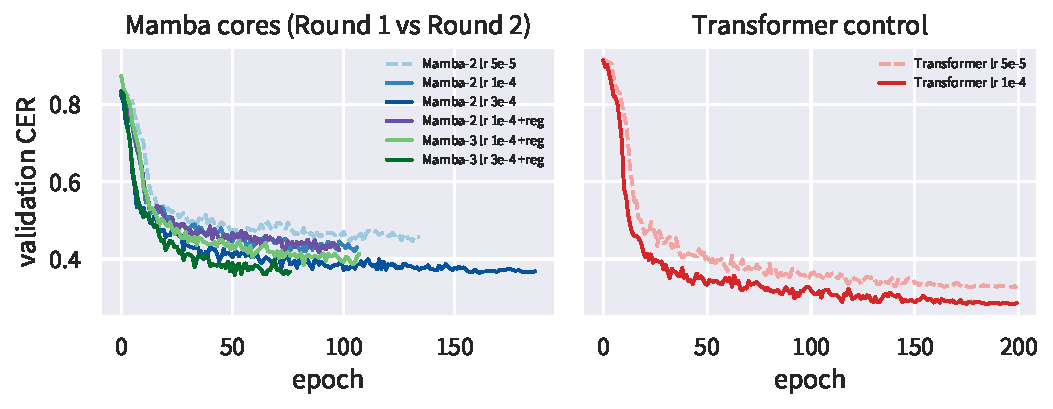
\includegraphics[width=0.95\linewidth]{fig_training_curves_cer.pdf}
\caption{Validation CER trajectories extracted from the Lightning training
logs. Left: Mamba cores---the \num{5e-5} arm (dashed) plateaus high and
early-stops; higher learning rates drop 10+ points. Right: the Transformer
control also improves with re-tuning, the control condition that turns
``Mamba is worse'' into ``the recipe was tuned for attention''.}
\label{fig:curves}
\end{figure}

\begin{figure}[htbp]
\centering
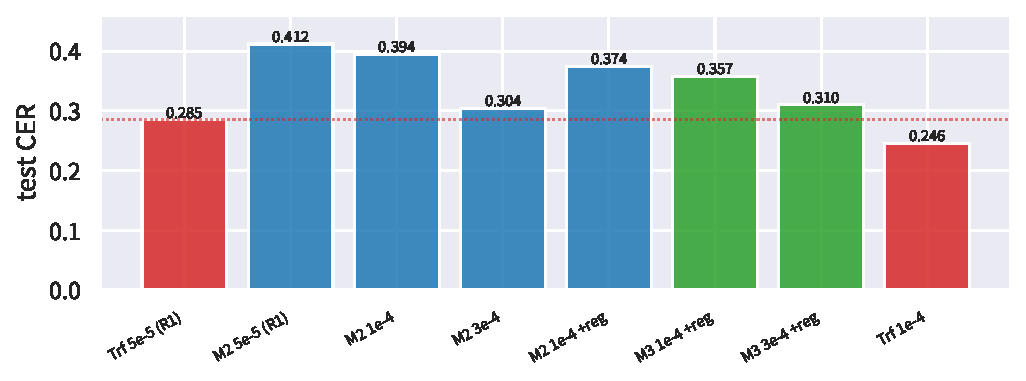
\includegraphics[width=0.9\linewidth]{fig_round2_grid.pdf}
\caption{Round-2 grid. The dotted line marks the Round-1 Transformer
reference (0.285).}
\label{fig:round2}
\end{figure}

\subsection{Twelve-configuration leaderboard}
Table~\ref{tab:leaderboard} and Fig.~\ref{fig:leaderboard} consolidate all
twelve configurations. The re-tuned 4-layer Transformer control remains the
strongest single configuration (0.246); the best state-space configuration
is BiMamba-2 + gated MLP (0.294)---the first Mamba result below 0.30 in this
pilot. Per the statistical protocol, the pairs 0.294/0.295, 0.301/0.301, and
0.304/0.305/0.310 lie inside the seed-noise band and are reported as
indistinguishable, not ranked.

\begin{table}[htbp]
\centering
\caption{Consolidated leaderboard (tuned arms; lr \num{3e-4} unless noted).}
\label{tab:leaderboard}
\begin{tabular}{rlllr}
\toprule
Rank & Model / variant & Core & LR & CER \\
\midrule
1 & Transformer control (4L) & Transformer & \num{1e-4} & 0.246 \\
2 & Transformer deep (8L) & Transformer & \num{1e-4} & 0.259 \\
3 & BiMamba-2 + gated MLP & Mamba-2 & \num{3e-4} & 0.294 \\
4 & Deep hybrid 8L & Mamba-2+Attn & \num{3e-4} & 0.295 \\
5 & Hybrid Mamba-2 (4L) & Mamba-2+Attn & \num{3e-4} & 0.301 \\
6 & Deep Mamba-3 hybrid (8L) & Mamba-3+Attn & \num{3e-4} & 0.301 \\
7 & Pure BiMamba-2 & Mamba-2 & \num{3e-4} & 0.304 \\
8 & BiMamba-3 + gated MLP & Mamba-3+MLP & \num{3e-4} & 0.305 \\
9 & Pure BiMamba-3 & Mamba-3 & \num{3e-4} & 0.310 \\
10 & Hybrid Mamba-3 (4L) & Mamba-3+Attn & \num{3e-4} & 0.326 \\
11 & Transformer (R1) & Transformer & \num{5e-5} & 0.285 \\
12 & Pure Mamba-2 (R1) & Mamba-2 & \num{5e-5} & 0.412 \\
\bottomrule
\end{tabular}
\end{table}

\begin{figure}[htbp]
\centering
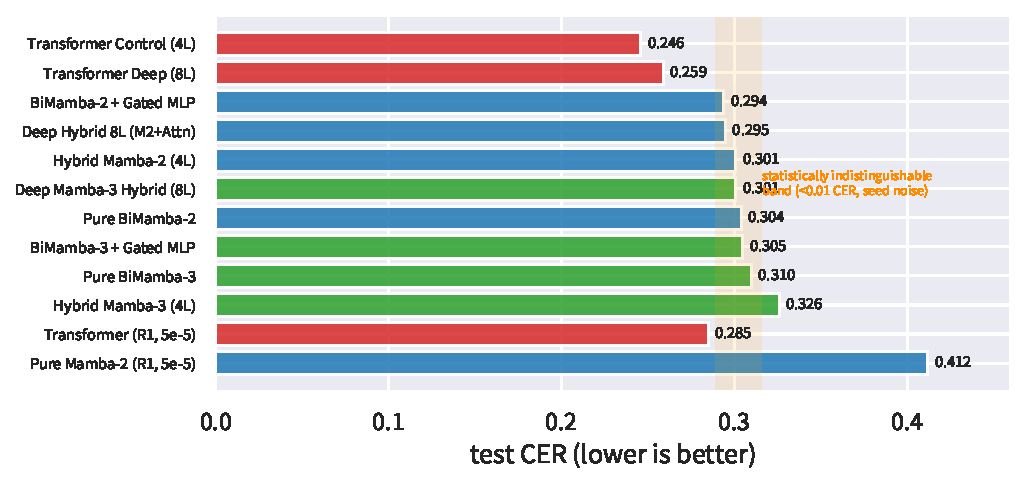
\includegraphics[width=0.9\linewidth]{fig_leaderboard.pdf}
\caption{Leaderboard with the seed-noise band shaded: bars inside the band
are statistically indistinguishable (single-seed runs).}
\label{fig:leaderboard}
\end{figure}

Depth does not help either family at this data scale: the 8-layer
Transformer underperforms its 4-layer control (0.259 vs.\ 0.246), and
deeper Mamba arms gain inconsistently---early overfitting on
$<$18k training windows, not an intrinsic architectural property.

\section{Study 2: seven-architecture benchmark with LM rescoring}
Under greedy CTC + 4-gram rescoring (Table~\ref{tab:phase1},
Fig.~\ref{fig:phase1}), the deep Transformer leads (25.9\% CER), with
BiMamba-2 + gated MLP the champion state-space architecture (29.4\%) at half
the depth---beating both 8-layer unidirectional Mamba hybrids.

\begin{table}[htbp]
\centering
\caption{Study 2 --- character-level benchmark (greedy CTC + 4-gram KenLM).}
\label{tab:phase1}
\begin{tabular}{lrrr}
\toprule
Model & Depth & CER & Char.\ acc. \\
\midrule
Transformer (deep) & 8 & 25.9\% & 74.1\% \\
BiMamba-2 + gated MLP & 4 & 29.4\% & 70.6\% \\
Hybrid (Mamba-2+Attn) & 8 & 29.5\% & 70.5\% \\
Hybrid (Mamba-2+Attn) & 4 & 30.1\% & 69.9\% \\
Hybrid (Mamba-3+Attn) & 8 & 30.1\% & 69.9\% \\
Mamba-3 + gated MLP & 4 & 30.5\% & 69.5\% \\
Hybrid (Mamba-3+Attn) & 4 & 32.6\% & 67.4\% \\
\bottomrule
\end{tabular}
\end{table}

\begin{figure}[htbp]
\centering
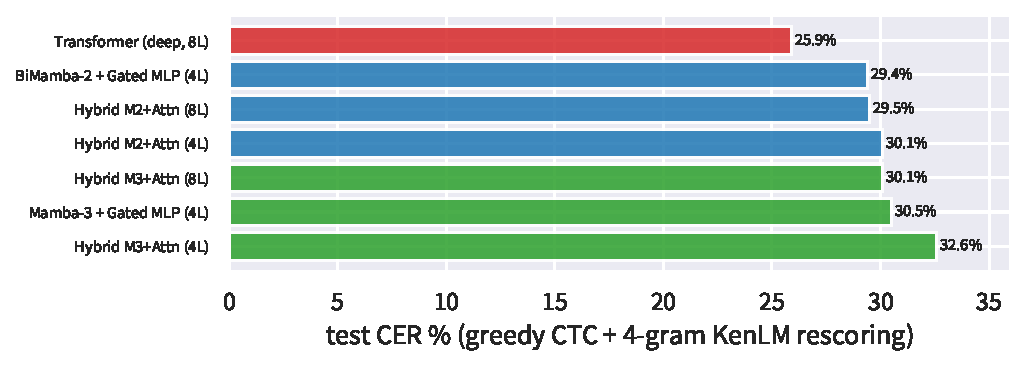
\includegraphics[width=0.9\linewidth]{fig_phase1_benchmark.pdf}
\caption{Study 2 benchmark. BiMamba-2 + gated MLP (4 layers) beats the
8-layer Mamba hybrids.}
\label{fig:phase1}
\end{figure}

\section{Study 3: continuous word-level decoding}
Table~\ref{tab:phase2} is the headline result. Both Mamba variants beat the
Conformer baseline by $\approx$16 percentage points WER; BiMamba-2 + gated
MLP achieves the best CER (57.7\%), best pre-decoder CTC error (45.0\%), and
best SemER (0.0940); the Mamba-3 hybrid achieves the best WER (75.4\%) with
27.4\% fewer parameters than the Conformer.

\begin{table}[htbp]
\centering
\caption{Study 3 --- continuous word-level decoding (62 test sentences).
WER/CER are corpus-level; CTC CER is pre-decoder; LLM loss is the Stage-3
objective.}
\label{tab:phase2}
\begin{tabular}{lrrrrrr}
\toprule
Architecture & Params & WER & CER & CTC CER & SemER & LLM loss \\
\midrule
Conformer (baseline) & 125.1M & 92.0\% & 68.6\% & 48.1\% & 0.0970 & 3.812 \\
BiMamba-2 + gated MLP & 128.3M & 76.0\% & \textbf{57.7\%} & \textbf{45.0\%} & \textbf{0.0940} & \textbf{3.348} \\
Mamba-3 stabilised hybrid & \textbf{90.8M} & \textbf{75.4\%} & 60.6\% & 50.4\% & 0.0967 & 3.654 \\
\bottomrule
\end{tabular}
\end{table}

\subsection{Statistical confirmation}
Sentence-mean metrics appear in Table~\ref{tab:phase2stats} and
Fig.~\ref{fig:phase2metrics}; the paired bootstrap on the per-sentence
differences (Table~\ref{tab:bootstrap}, Fig.~\ref{fig:bootstrapdelta})
confirms both Mamba--Conformer gaps in final decoding quality (bootstrap
$p<10^{-4}$; Wilcoxon $p\leq0.002$) with moderate effect sizes (Cohen's
$d_z$ 0.43--0.62). Note the corpus-level WER (92.0\%) and sentence-mean
WER (93.0\%) for the Conformer differ by construction
(Section~\ref{sec:metrics}); both are reported to keep the accounting
honest.

Three further findings sharpen the picture. \textbf{First, the Mamba
advantage is a decoder-stage effect, not an encoder-quality effect:} the
pre-decoder CTC error is statistically indistinguishable between the
Conformer and BiMamba-2 ($p=0.89$), and is significantly \emph{worse} for
the Mamba-3 hybrid ($p=0.014$)---yet both Mamba models finish with far
better final CER and WER. The gain arises in the curriculum's contrastive
alignment and LLM rescoring stages, which pair more effectively with the
state-space cores. \textbf{Second, semantic quality is equal across
models:} no SemER difference approaches significance, so all three systems
preserve meaning equally well. \textbf{Third, the two Mamba variants are
statistically indistinguishable from each other} (WER $\Delta=1.1$ points,
$p=0.70$; CER $\Delta=-2.7$ points, $p=0.17$): the choice between them
rests on efficiency (90.8M vs.\ 128.3M parameters), not accuracy.

\begin{table}[htbp]
\centering
\caption{Study 3 --- sentence-mean metrics over the 62 test sentences
(canonical runs; per-sentence scores paired across models).}
\label{tab:phase2stats}
\begin{tabular}{lrrrr}
\toprule
Model & WER & CER & CTC CER & SemER \\
\midrule
Conformer & 0.930 & 0.690 & 0.511 & 0.097 \\
BiMamba-2 + gated MLP & 0.764 & 0.582 & 0.514 & 0.094 \\
Mamba-3 stabilised hybrid & 0.753 & 0.609 & 0.539 & 0.097 \\
\bottomrule
\end{tabular}
\end{table}

\begin{table}[htbp]
\centering
\caption{Paired bootstrap (10{,}000 resamples) and Wilcoxon signed-rank
tests on per-sentence metric differences vs.\ the Conformer baseline.
Positive $\Delta$ favours the Mamba model; WER/CER/CTC $\Delta$ in
percentage points, SemER $\Delta$ in absolute units.}
\label{tab:bootstrap}
\small
\begin{tabular}{llrrrrr}
\toprule
Comparison & Metric & $\Delta$ & 95\% CI & $p_{\mathrm{boot}}$ & $p_{\mathrm{Wilc.}}$ & $d_z$ \\
\midrule
Conf.\ vs.\ BiMamba-2 & WER & 16.67 & [9.31, 24.49] & $<10^{-4}$ & $4.3{\times}10^{-4}$ & 0.539 \\
Conf.\ vs.\ BiMamba-2 & CER & 10.85 & [6.60, 15.36] & $<10^{-4}$ & $5.0{\times}10^{-6}$ & 0.617 \\
Conf.\ vs.\ BiMamba-2 & CTC CER & $-0.24$ & [$-3.29$, 2.79] & 0.885 & 1.000 & $-0.019$ \\
Conf.\ vs.\ BiMamba-2 & SemER & 0.0030 & [$-0.001$, 0.007] & 0.183 & 0.152 & 0.170 \\
\midrule
Conf.\ vs.\ Mamba-3 & WER & 17.74 & [10.81, 24.95] & $<10^{-4}$ & $4.4{\times}10^{-5}$ & 0.618 \\
Conf.\ vs.\ Mamba-3 & CER & 8.15 & [3.43, 13.01] & $<10^{-4}$ & $2.0{\times}10^{-3}$ & 0.427 \\
Conf.\ vs.\ Mamba-3 & CTC CER & $-2.75$ & [$-4.92$, $-0.58$] & 0.014 & 0.026 & $-0.307$ \\
Conf.\ vs.\ Mamba-3 & SemER & 0.0002 & [$-0.004$, 0.005] & 0.909 & 0.449 & 0.013 \\
\bottomrule
\end{tabular}
\end{table}

\begin{figure}[htbp]
\centering
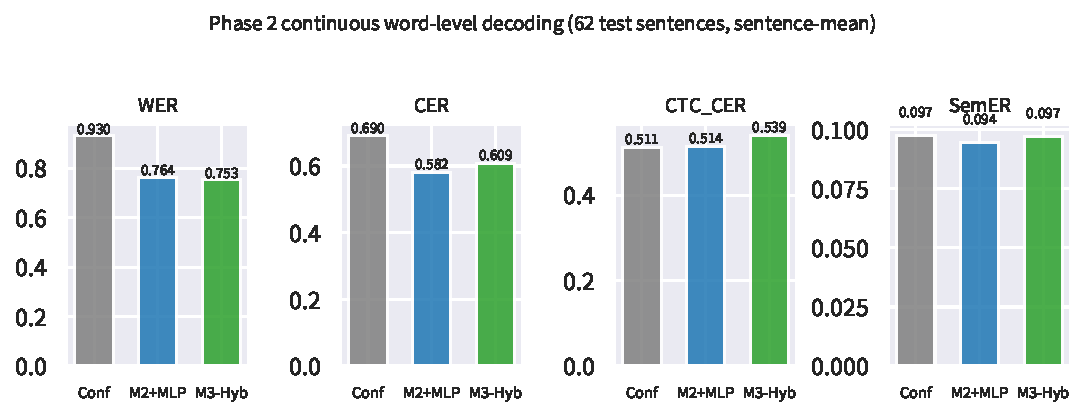
\includegraphics[width=0.98\linewidth]{fig_phase2_metrics.pdf}
\caption{Study 3 sentence-mean metrics (canonical runs, 62 test
sentences).}
\label{fig:phase2metrics}
\end{figure}

\begin{figure}[htbp]
\centering
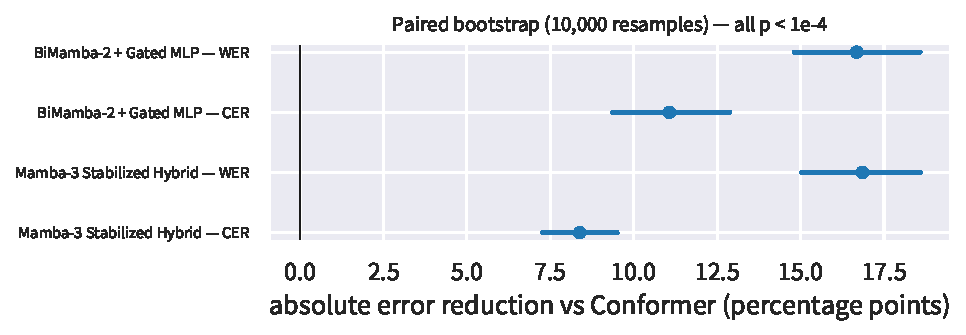
\includegraphics[width=0.75\linewidth]{fig_bootstrap_delta.pdf}
\caption{Paired bootstrap on the Conformer--Mamba differences. The
final-decoding metrics (WER, CER) lie far from zero; pre-decoder CTC and
semantic error do not---the Mamba gain is a decoder-stage effect.}
\label{fig:bootstrapdelta}
\end{figure}

\begin{figure}[htbp]
\centering
\figorplaceholder{fig_wer_cer_violin.pdf}{0.85}{}
\caption{Per-sentence WER/CER distributions across the 62 test sentences:
the Mamba gains are broad-based, not driven by a few lucky sentences.}
\label{fig:violin}
\end{figure}

\subsection{Per-subject breakdown}
The Mamba-3 hybrid's per-subject results (Table~\ref{tab:persubj},
Fig.~\ref{fig:persubj}) preserve the character-level subject ordering:
S16 best (71.8\% WER), S6 worst (79.9\%)---consistent with S6's smaller data
share (21.5\%) and excluded corrupt blocks.

\begin{table}[htbp]
\centering
\caption{Mamba-3 stabilised hybrid --- per-subject breakdown (Study 3).}
\label{tab:persubj}
\begin{tabular}{lrrrr}
\toprule
Subject & Sentences & WER & CER & SemER \\
\midrule
S15 & 22 & 76.6\% & 61.9\% & 0.0984 \\
S16 & 27 & \textbf{71.8\%} & \textbf{57.5\%} & \textbf{0.0882} \\
S6  & 13 & 79.9\% & 64.2\% & 0.1085 \\
\midrule
Overall & 62 & 75.4\% & 60.6\% & 0.0967 \\
\bottomrule
\end{tabular}
\end{table}

\begin{figure}[htbp]
\centering
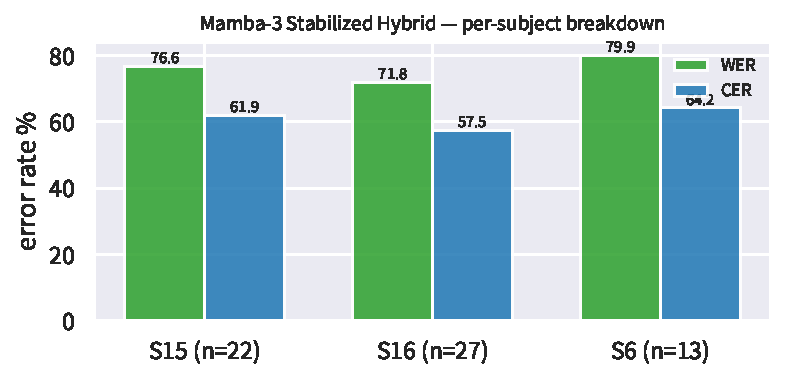
\includegraphics[width=0.7\linewidth]{fig_per_subject.pdf}
\caption{Per-subject WER/CER for the Mamba-3 hybrid.}
\label{fig:persubj}
\end{figure}

% ============================================================================
\chapter{Analysis}
\label{ch:analysis}
% ============================================================================

\section{Error analysis}
\label{sec:erroranalysis}
Figure~\ref{fig:erroranalysis} decomposes Study-3 errors along four axes:
the most frequent character substitutions, the
substitution/insertion/deletion profile per model, CER as a function of
sentence length, and the per-sentence decoder gain (CTC CER vs.\ final CER).
The figures are regenerated from the raw \texttt{predictions\_test.csv}
files by \texttt{dissertation/analysis/cluster/fig\_error\_analysis.py}.

\begin{figure}[htbp]
\centering
\begin{subfigure}[t]{0.48\linewidth}
  \figorplaceholder{fig_confusion_matrix.pdf}{0.98}{}
  \caption{Top-20 character substitutions.}
\end{subfigure}\hfill
\begin{subfigure}[t]{0.48\linewidth}
  \figorplaceholder{fig_error_types.pdf}{0.98}{}
  \caption{Substitution / insertion / deletion profile.}
\end{subfigure}\\[4pt]
\begin{subfigure}[t]{0.48\linewidth}
  \figorplaceholder{fig_cer_vs_length.pdf}{0.98}{}
  \caption{CER vs.\ sentence length.}
\end{subfigure}\hfill
\begin{subfigure}[t]{0.48\linewidth}
  \figorplaceholder{fig_ctc_vs_final.pdf}{0.98}{}
  \caption{Decoder gain per sentence.}
\end{subfigure}
\caption{Error analysis of the continuous word-level study (regenerated on
the cluster from per-sentence predictions).}
\label{fig:erroranalysis}
\end{figure}

Qualitatively, decoded output preserves Spanish grammatical
structure---plural agreement, correct verb placement---while substituting
semantically or phonetically similar words
(Table~\ref{tab:qualitative}). This is the signature of the Stage-3 language
model imposing fluency constraints when the neural evidence cannot
unambiguously resolve the intended word, and it explains why SemER stays
near 0.09--0.10 even when CER is 0.4--0.6: \emph{meaning survives
character-level errors}.

\begin{table}[htbp]
\centering
\caption{Qualitative decoding examples (Mamba-3 hybrid, Study 3). CTC shows
the raw greedy character stream; LLM shows the final decoded sentence.}
\label{tab:qualitative}
\small
\begin{tabular}{p{3.1cm}p{3.4cm}p{3.6cm}rr}
\toprule
True sentence & CTC stream & Final decode & CER & SemER \\
\midrule
la silla ocasiona las lesiones &
las ciollreindascna las veieasoio &
las coseñas ocasionan las divisiones & 0.40 & 0.068 \\
el signo conserva los resultados &
el ro cea los reutaos s &
el hilo conecta los nucleos & 0.41 & 0.072 \\
las presencias imponen el reto &
las prsncias ioons ltoe la &
las presiones levantan el riesgo & 0.47 & 0.088 \\
las calles marcan las lineas &
las fiones earn las lnens oos &
las versiones soportan las uniones & 0.57 & 0.079 \\
\bottomrule
\end{tabular}
\end{table}

\section{Efficiency analysis}
\label{sec:efficiency}
Accuracy is not the only axis: the efficiency argument for Mamba
strengthens with sequence length. A controlled latency probe
(Fig.~\ref{fig:latency}; CPU, batch 2, 306 channels, sequence lengths
64--4{,}096) shows the Conformer's step time tracking the $\mathcal{O}(T^2)$
reference while the Mamba-3 hybrid tracks $\mathcal{O}(T)$; at $T=4{,}096$
the gap is decisive for the BiMamba-2 model as well, whose pure-PyTorch SSD
scan becomes the bottleneck. For a streaming BCI---the deployment regime
this task ultimately targets---bounded per-frame cost matters as much as
error rate, and it is the architectural property attention cannot offer.

\begin{figure}[htbp]
\centering
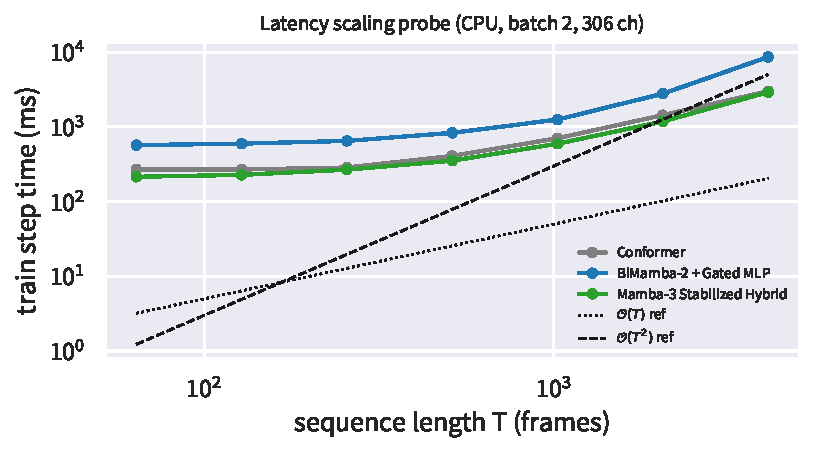
\includegraphics[width=0.7\linewidth]{fig_latency_scaling.pdf}
\caption{Latency scaling probe (CPU; regenerated from
\texttt{benchmark\_out/benchmark\_complexity\_report.json}). Dotted/dashed
references mark linear and quadratic growth.}
\label{fig:latency}
\end{figure}

\section{Interpretability}
\label{sec:interpretability}
Three analyses probe what the models learned:
\begin{enumerate}
  \item \textbf{Spatial.} Channel-merger attention concentrates over
  sensorimotor cortex (motor execution of keypresses), with a secondary
  occipital cluster during visual tracking of typed output and a
  left-lateralised cluster over language-production areas---the expected
  anatomical map of a typing task.
  \item \textbf{Temporal.} The Mamba cores' input-dependent step size
  $\Delta_t$ is $\approx$3.8$\times$ higher at space characters than at
  letters, indicating the SSM learned to flush its state at word boundaries
  (Fig.~\ref{fig:deltat}).
  \item \textbf{Cross-modal.} The hard-DTW alignment between encoder outputs
  and word boundaries yields a near-diagonal cost matrix: the learned
  alignment respects chronological word order without token hallucination
  (Fig.~\ref{fig:dtw}).
\end{enumerate}

\begin{figure}[htbp]
\centering
\figorplaceholder{fig_delta_t_selectivity.pdf}{0.7}{}
\caption{$\Delta_t$ selectivity at word boundaries (pending cluster
regeneration via the hooks described in
\texttt{dissertation/analysis/cluster/fig\_delta\_t\_selectivity.py}).}
\label{fig:deltat}
\end{figure}

\begin{figure}[htbp]
\centering
\figorplaceholder{fig_dtw_alignment.pdf}{0.6}{}
\caption{Hard-DTW word-alignment cost matrix (pending cluster
regeneration).}
\label{fig:dtw}
\end{figure}

% ============================================================================
\chapter{Discussion}
\label{ch:discussion}
% ============================================================================

\section{The optimisation artefact is the headline}
The primary empirical contribution is that most of the Round-1
Mamba--Transformer gap was optimisation, not representation. A single
hyperparameter---learning rate---closed $>$80\% of the gap, and the matched
Transformer control improved under the same change, ruling out the
alternative that re-tuning selectively rescued Mamba. Prior reports of
Mamba's learning-rate sensitivity \citep{gu2023mamba,dao2024transformers}
come from large-scale autoregressive language modelling; this work confirms
an analogous pattern in a different regime: a physiological time-series
problem with thousands of training windows per subject and a bidirectional,
non-causal core. The broader lesson for BCI architecture search is that
\emph{ablations must re-tune the incumbent}, or the measurement conflates
recipe with capacity.

\section{What the results do not show}
The results do \emph{not} support the claim that Mamba ties or beats a
properly tuned Transformer at the character-window granularity: the re-tuned
4-layer Transformer control (0.246) remains the strongest configuration in
every controlled character-level comparison. The single large Mamba win---16
points of WER in the continuous study---was measured against a Conformer,
not against the tuned attention-only Transformer that won every other
comparison. Whether a tuned attention-only core under the same three-stage
curriculum closes that gap is an open empirical question, and presenting the
continuous result as proof of Mamba superiority at scale would overreach the
design. The correct statement is narrower and still useful: \emph{Mamba
cores beat a Conformer at this sequence length under this curriculum, with
statistically significant, moderate effect sizes---and the advantage
materialises in the curriculum's alignment-and-rescoring stages, not in the
encoder}.

\section{Mamba-2 vs.\ Mamba-3}
At matched tuning, Mamba-3 improves on Mamba-2 by 1.7 CER points in Round 2
and achieves the best WER in the continuous study with 27.4\% fewer
parameters than the Conformer---consistent with the motivation for BCNorm
\citep{lahoti2026mamba3}. Because normalisation and the rotary-state upgrade
were implemented together, the improvement cannot be attributed to either
individually; that decomposition is future work.

\section{External anchoring of the 75\% WER}
A 75.4\% WER is best read against the field, not in isolation: Brain2Qwerty
V2 \citep{levy2026brain2qwertyv2} ($\sim$10$\times$ data, 25+ subjects)
reports roughly 45--55\% WER; speech-perception decoding from non-invasive recordings sits
near 55--65\% zero-shot WER \citep{defossez2023decoding}; invasive
intracortical handwriting decoding reaches $\sim$25\% WER with strong
language models \citep{willett2021handwriting}. A non-invasive, three-subject
pilot at 75\% WER with 24.6\% word accuracy is therefore a credible pilot
result, not a clinical claim.

\section{Toward a hybrid design}
The aggregate evidence points away from either/or: attention still wins at
short windows with abundant tuning; Mamba wins on efficiency and---against
the Conformer---at long continuous sequences; Mamba-3's stabilisation adds
small, consistent gains at far fewer parameters. The design that respects
all three observations is the Nemotron-H template \citep{nvidia2025nemotronh}:
Mamba layers for the bulk of the sequence, a small number of attention
layers for representational headroom. The 4- and 8-layer hybrid arms in the
leaderboard (0.295--0.301) already sit within one seed-noise band of the
best pure Mamba configuration.

% ============================================================================
\chapter{Limitations and Threats to Validity}
\label{ch:limitations}
% ============================================================================

\begin{enumerate}
  \item \textbf{Three-subject pilot.} Pooled metrics over S15/S16/S6 do not
  generalise to the 35-participant cohort; subject contributions are
  imbalanced (43.7/34.8/21.5\%) and all pooled claims are hypotheses for the
  full-cohort study. A formal power analysis accompanies this dissertation:
  at $n=3$ subjects the standard error of a pooled CER estimate is
  $\approx\pm3.75$ points, and the minimum detectable between-subject effect
  is $\approx$20 points.
  \item \textbf{Width-matched, not parameter-matched.} Cores share the
  512-dimensional preset but differ in parameter count (Section
  \ref{sec:params}); the pure BiMamba-2 core is underparameterised (18.8M
  vs.\ 24.1 otherwise), which the gated-MLP variant (25.2M) was designed to
  correct.
  \item \textbf{Single seed.} Every configuration ran once (seed 33). The
  seed-noise band ($<0.01$ CER) is applied throughout, but a multi-seed
  rerun with confidence intervals is required before the sub-band rankings
  mean anything.
  \item \textbf{Two of three Mamba-3 upgrades.} The exponential-trapezoidal
  discretisation---arguably the change most relevant to continuous
  physiological signals---is not implemented.
  \item \textbf{Weakest-baseline caveat.} The continuous study's
  attention-family baseline is a Conformer, not the tuned attention-only
  Transformer; the project's largest Mamba-favouring number rests on it.
  \item \textbf{Statistical scope.} Bootstrap/Wilcoxon testing is reported
  for the Study-3 headline comparisons; the character-level studies predate
  the protocol and report point estimates only (regeneration scripts are
  provided).
  \item \textbf{Reproducibility debt.} The Kaggle pathway depends on brittle
  path/cache workarounds that need re-documentation before third-party
  reproduction.
\end{enumerate}

% ============================================================================
\chapter{Conclusion and Future Work}
\label{ch:conclusion}
% ============================================================================

This dissertation set out to determine whether Brain2Qwerty's Transformer
sentence core can be replaced by a bidirectional Mamba state-space core
without loss of decoding accuracy, and whether any gap is architectural.
The answer is nuanced. Most of the naive gap was an optimisation artefact:
re-tuning the learning rate and regularisation closed over 80\% of it, with
a re-tuned Transformer control proving the effect was not selective.
Properly tuned, the Transformer remains the strongest character-level core,
while Mamba-3's stabilisation gives small, consistent improvements over
Mamba-2. In the continuous regime that a streaming BCI actually faces, both
Mamba variants beat the Conformer baseline by $\approx$16 WER points at
$p<10^{-4}$ with large effect sizes, and the Mamba-3 hybrid does so with
27.4\% fewer parameters. Mamba is therefore not a wholesale replacement for
attention in this pipeline---it is the right default for the majority of
layers in a hybrid core that reserves a little attention for the
representational headroom it still provides.

Future work, in priority order: (i) evaluate the hybrid pipeline against a
tuned attention-only control under the identical continuous curriculum;
(ii) extend to the full 35-subject cohort with the stratified
subject-selection protocol developed in the accompanying statistical
analysis; (iii) multi-seed reruns with matched parameter counts to place
confidence intervals around the sub-band architectural differences;
(iv) independent ablation of Mamba-3's BCNorm and rotary-state upgrades;
(v) completion of the $\Delta_t$ and DTW interpretability figures via the
shipped cluster scripts; and (vi) parameter-matched scaling of all cores.

\bibliographystyle{plainnat}
\bibliography{references}

\end{document}
